\documentclass[10pt, conference, compsocconf]{IEEEtran}
\hyphenation{op-tical net-works semi-conduc-tor}

\usepackage{cite}
\usepackage{epsfig}
\usepackage{graphicx}
\usepackage{subfigure}
\usepackage{algorithmic}

\begin{document}
\bibliographystyle{IEEEtran}

\title{MALMOS: Machine Learning-based Mobile Offloading Scheduler with Online
Training}


\author{\IEEEauthorblockN{Heungsik Eom, Renato Figueiredo}
\IEEEauthorblockA{Advanced Computing and Information Systems Laboratory\\
Electrical and Computer Engineering\\
University of Florida, Gainesville, Florida, USA\\
\{hseom, renato\}@acis.ufl.edu}
\and
\IEEEauthorblockN{Huaqian Cai, Gang Huang}
\IEEEauthorblockA{Operating System and Middleware Laboratory\\
School of Electronics Engineering and Computer Science\\
Peking University, Beijing, China\\
\{caihq12, hg\}@pku.edu.cn}
}

\maketitle

\begin{abstract}
%
This paper proposes and evaluates a novel framework for the mobile
offloading scheduler, MALMOS, which is based on online, runtime machine
learning techniques.
%
In contrast to previous works which rely on application-dependent
parameters or predefined scheduling policies, MALMOS provides an online
training mechanism for the machine learning-based runtime scheduler such
that it supports a policy that dynamically adapts scheduling decisions
based on the observation of previous offloading decisions at runtime.
%
To demonstrate its practical applicability, we integrated MALMOS with an
existing Java-based, offloading-capable code refactoring framework,
DPartner.
%
Using this integration, we performed quantitative experiments to
evaluate the performance and cost for three machine learning
algorithms: instance-based learning, perceptron, and na\"{i}ve bayes,
with respect to classifier training time, classification time, and
scheduling accuracy.
%
Our evaluation present that instance-based leaning and perceptron show
higher than 80\% of the scheduling accuracy with the reasonably
acceptable overhead.
%
%In this paper, we present an OpenCL-based remote offloading framework
%designed for mobile platforms by shifting the motivation and
%advantages of using the OpenCL framework for the HPC cluster environment
%into mobile cloud computing where OpenCL workloads can be exported from
%a mobile node to the cloud.
%
%Furthermore, our offloading framework handles service discovery, access
%control, and data privacy by building the framework on top of a social
%peer-to-peer virtual private network, SocialVPN. 
%
%We developed a prototype implementation and deployed it into local- and
%wide-area environments to evaluate the performance improvement and
%energy implications of the proposed offloading framework.
%
%Our results show that, depending on the complexity of the workload and
%the amount of data transfer, the proposed architecture can achieve more
%energy efficient performance by offloading than executing locally.
\end{abstract}

\begin{IEEEkeywords}
Mobile platform, computation offloading, machine learning, runtime
scheduler, online training
\end{IEEEkeywords}

\section{Introduction}
%
Over the last decade, mobile offloading techniques have emerged as
a means to overcome resource constraints of mobile platforms (i.e.
smartphones, tablets).
%
Offloading allows these devices to delegate computationally-intensive
tasks to more powerful external resource, such as personal workstations
or cloud servers.
%
Initially, research interests on mobile offloading techniques
have focused on core mechanisms that deal primarily with \textit{what to
offload} and \textit{how to offload}.
%
The research community has studied various approaches to implement mobile
offloading frameworks which fall in the following categories:
application partitioning~\cite{maui, cuckoo}, thread
migration~\cite{clonecloud, comet}, application migration~\cite{hung},
and distributed offloading frameworks~\cite{serendipity}.\\
%
\indent However, one important fact is that benefits and drawbacks
from offloading computation-intensive portions of mobile applications
can be influenced by various internal and external factors, such as
applications requirements, network conditions, and computing
capabilities of mobile and external devices. 
%
Thus, \textit{whether to offload or execute locally} needs to be
decided dynamically, and the decision-making can benefit from monitoring
the aforementioned dynamic features at runtime.
%
Otherwise, incorrect offloading decisions may cause performance
degradation and/or increase energy consumption.
%
Related work has also considered dynamic scheduling for mobile
offloading frameworks.
%
For example, Kwon et al.~\cite{kwon} consider a simple rule-based
scheduler in which the framework decides to offload  mobile
computations only when the data transfer size is higher than a certain
threshold.
%
MAUI~\cite{maui} utilizes a linear regression model using predefined
features to make offloading decisions.\\
%
\indent Even though these systems consider runtime schedulers for mobile
offloading, which take dynamic features such as data transfer size or
network conditions into account to make offloading decisions, it is
impractical for these approaches to build a generic offloading decision
policy embracing all possible cases over dynamic mobile environments.
% 
Furthermore, it is difficult to generally apply the above efforts to
various applications, since each application has its own requirements or
characteristics.
%
For example, gaming and image processing application may have different
computation complexity, though they process a similar size of data.\\
%
%Therefore, in practice, the mobile offloading scheduler has to work
%independently with the type of applications without any predefined
%decision rules.\\ 
%
\indent In this paper, we aim to develop a general framework for an
adaptive scheduler for mobile offloading by employing online, runtime
machine learning techniques, MALMOS which stands for machine
learning-based mobile offloading scheduler.
%
In this approach, a machine learning classifier makes decisions of
whether mobile computations should be offloaded to external resources,
or executed locally. 
%
To this end, we extend our previous work on offline machine
learning-based runtime scheduler~\cite{ml}, and develop a novel online
scheduling module in which any appropriate machine learning classifier
can be utilized for the runtime offloading scheduler.
%
First, we define application programming interfaces (APIs) to monitor and
acquire dynamic features, such as data sizes, network latency and
bandwidth, and the status of external devices.
%
Furthermore, MALMOS provides an online training mechanism for
the machine learning-based runtime scheduler such that it supports a
policy that dynamically adapts scheduling decisions at runtime based on
the observation of previous offloading decisions.\\ 
%
\indent To demonstrate its practical applicability, we integrated MALMOS
with an existing Java-based, offloading-capable code refactoring
framework, \textit{DPartner}~\cite{dpartner}.
%
Originally, the offloading-capable mobile applications generated by
DPartner depend on static (or user-provided) input to decide whether to
execute offloadable computations (i.e. Java classes) locally or remotely.
%
By combining this paper's machine learning-based runtime scheduler with
these applications, offloading decisions are dynamic and do not require
user input.
%
We have implemented an online-scheduled DPartner prototype, and used it
to perform quantitative experiments with Android mobile devices and
applications to quantitatively evaluate the cost and performance for
three machine learning algorithms: instance-based learning, perceptron,
and na\"{i}ve bayes.
%
These are evaluated with respect to classifier training time,
classification time, and scheduling accuracy.
%
Even though there have been prior related studies which suggest
utilizing machine learning techniques for mobile computing environments,
to the best of our knowledge, our work is the first to consider an
online training mechanism for the machine learning-based runtime
scheduler, and to demonstrate with a end-to-end system performance and
cost of various machine learning algorithms for the runtime scheduler of
mobile offloading tasks.\\
%
\indent The rest of the paper is organized as follows.
%
In Section II, we overview prior research efforts on 
mobile offloading frameworks as well as the use of machine
learning techniques for scheduling problems from various domains.
%
Section III summarizes our previous work which proposed the machine
learning based runtime scheduler for mobile offloading framework and
motivates the concept of the online training mechanism for MALMOS. 
%
In Section IV and V, we explain and evaluate our implementation of
MALMOS with the online training mechanism.
%
Section VI describes the current and potential applications for
our work.
%
Finally, we conclude the paper in Section VII.
%
\section{Related Works}
%
\subsection{Adaptive Mobile Offloading Frameworks}
%
Many approaches on adaptive mobile offloading framework have been
proposed to address scheduling problems on dynamic environments.
%
In ~\cite{shigeru}, a prediction heuristic uses linear functions to
estimate the local and remote processing time as well as the data
transfer time.
%
The remote server updates these linear functions using least-squares
method and returns the updated prediction functions to the mobile client,
then these functions are used to compare the performance between local
processing and offloading.
%
Gu et al.~\cite{xiaohui} try to relieving the memory restriction of the
mobile device by adaptively making offloading decisions with help from
the fuzzy control model, called Offloading Inference Engine (OLIE).
%
OLIE monitors the available memory margin of the mobile device and
network bandwidth, and maps them into the offloading decision
specifications defined by the application developer so that when the
present condition matches the specified rule, the mobile workloads are
offloaded to the remote server.
%
Kwon et al.~\cite{kwon} consider a simple rule-based
scheduler in which the framework decides to offload the mobile
computation only when the data transfer size is higher than a certain
threshold.\\
%
\indent Although the aforementioned studies take dynamic features
from hardware or network level (i.e. available memory size, network
bandwidth) into account, they still depend on the predefined static
decision rules or cost models while preventing the scheduler from
adapting to dynamic conditions on runtime.
%
In contrast, our approach do not rely on any predefined specifications
or prior knowledge of the mobile application.
%
Instead, we consider machine learning techniques for the adaptive mobile
offloading scheduler in which the scheduler can be trained on and 
dynamically make offloading decisions on runtime. 
%
\subsection{Machine Learning Techniques for Runtime Scheduler}
%
Various areas such as heterogeneous computing platforms, grid computing
systems, and data center have used machine learning techniques to
address dynamic scheduling problems.
%
In~\cite{zheng}, machine learning techniques are used to provide a
compiler-based, automatic and portable predictor for multi-core
processors.
%
In order to decide the optimal number of threads and scheduling policy,
the framework used a feed-forward artificial neural network and a
multi-class support vector machine model, respectively.
%
Berral et al.~\cite{josep} propose an energy-aware
data center through server consolidation by turning off idle servers
with assistance from machine learning based scheduling.
%
The scheduler predicts the future performance of the jobs and power
consumption in the resulting job allocation using linear regression
algorithms.
%
This framework uses artificial neural networks for the performance
modeler which predicts task computation and data communication costs,
and this modeler is used by the directed acyclic graph to determine an
appropriate schedule.\\
%
\indent Along with the machine learning-based runtime scheduler, we
further consider the adaptive online training mechanism which stretches
and shrinks the length of the training period according to the scheduling
accuracy.
%
\section{Runtime Scheduler for Mobile Offloading System}
%
In this section, we summarize our previous work on the machine
learning-based runtime scheduler for mobile offloading framework in
which we noticed offloading performance dependency on various dynamic
features and suggested applying machine learning techniques to the
runtime scheduler for mobile offloading framework by showing the
performance and cost among various machine learning algorithms.
%
Then, we describe the challenge on the online training mechanism for the
machine learning-based runtime scheduler.
% 
\subsection{Offloading Performance}
%
In our previous work~\cite{ml}, we validated the necessity and efficacy
of the runtime scheduler for mobile offloading framework through
detailed measurement experiments.
%
With the OpenCL-based mobile offloading framework~\cite{ocloff}, we
performed various experiments using four different OpenCL workload
kernels used in a variety of areas such as image processing filters and
mathematical simulations.
%
Also, in order to observe the impact of different network conditions on
the offloading performance, we configured different network conditions:
local area network, campus network, and wide area network (i.e. Amazon
EC2 cloud).
%
In the evaluation, we verified that different network conditions cause
significantly different offloading performance.
%
In most cases, offloading to the remote resource located in local area
network has better performance than local processing in four OpenCL
workload kernels used for the experiments.
%
In contrast, offloading to the remote resource located in campus network
and Amazon EC2 cloud, where have much limited network conditions than
local area network, can exhibit longer execution time than local
processing according to the size of data transfer.\\ 
%
\indent It is worth noting that each OpenCL workload kernel shows
the different performance, even though they process the similar size of
data.
%
This is because each kernel has different computational complexities so
they gain the different amount of performance improvement while paying
the same cost to send the data to the remote resource.
%
These results show that there exists the offloading performance
variation over different network conditions and OpenCL workload kernels.
%
Consequently, proper scheduling can have a significant impact on the
offloading performance and mobile offloading framework requires the
support from the runtime scheduler.
%
\subsection{Machine Learning-based Runtime Scheduler}
%
Based on our observation, we applied machine learning techniques to the
runtime scheduling problem for mobile offloading framework.
%
For doing this, we first chose a set of relevant attributes which have
an impact on making offloading decisions.
%
Also, by running the OpenCL-based offloading framework with different
network configurations, OpenCL workload kernels, and data size, we
collected a total 640 data instances to train and test the classifiers
of various machine learning algorithms.
%
Using the gathered dataset, we trained various machine learning
classifiers with \textit{Weka}, a Java-based open source package for
machine learning techniques.
%
Finally, we implemented the machine learning-based runtime scheduler by
building the trained machine learning classifiers onto the
OpenCL-based mobile offloading system.\\
%
\indent In order to evaluate the machine learning-based runtime
scheduler for mobile offloading framework, we deployed the OpenCL-based
offloading system under various network bandwidth controlled by a
network characteristic tool called \textit{Traffic Control} (TC).
%
In our evaluation, we observed that most of the machine learning-based
schedulers show the reasonably high scheduling performance by achieving
higher than 80\% of the scheduling accuracy.
%
Especially, Instance-Based Learning has the most accurate scheduling
performance among various schedulers showing 92\% of the scheduling
accuracy.
%
Compared with other machine learning-based schedulers, furthermore,
Instance-Based Learning exhibits a fairly small penalty, which is the
additional cost in terms of the execution time and energy consumption
when the scheduler makes incorrect decisions.
%
%\section{Challenge on Online Training for Machine Learning-based Mobile
%Offloading Scheduler}
%
%The main goal of MALMOS is to construct the machine learning-based
%runtime scheduler with online training for mobile offloading framework.
%
%In this section, we explain the difference between offline and online
%training for the machine learning technique.
%
%Also, we describe the challenge on the online training mechanism for the
%machine learning-based runtime scheduler.
%
\subsection{Offline vs. Online Training}
%
%Machine learning technique is a branch of artificial intelligence
%through which a system can learn from previous experiences proactively
%and predict the future actions of the target system.
%
In fact, there exist two possible ways to train the machine learning
classifier: \textit{offline} and \textit{online} training.
%
In offline training, the machine learning classifier can be trained
using a set of the pre-collected static data.
%
Once the machine learning classifier is trained in the initial training
phase, the classifier does not change its prediction behavior.
%
It is therefore difficult to reflect the unseen situations or conditions
which have not been trained in the initial training phase.
%
For that reason, offline machine learning should be trained through a
large set of data which covers as many cases as possible in order to
accomplish high prediction performance.\\
%
\indent On the other hand, the online machine learning technique does
not depend on any pre-trained classifiers to approximate or predict 
the future behaviors of the target system.
%
Instead, online machine learning trains its classifier at a time
when a new data instance arrives in.
%
More specifically, the classifier of online machine learning is trained
whenever the result of the comparison between the prediction and actual
behavior is available.
%
Thus, the main challenge of online machine learning is to deliver the
prediction correctness into the training process, so that it can train
the classifier continuously based on the prediction correctness feedback.
%
%\subsection{Requirement for Online Training Machine Learning-based
%Mobile Offloading Scheduler}
%
%As mentioned in the previous subsection, the online training mechanism has
%to maintain its own continuous feedback channel from the examination of
%whether the prediction made by the classifier is correct, and if not,
%which prediction should have made.  
%
However, it can be too expensive to figure out the correct prediction,
since the system may have to attempt all of the possible predictions to
know which prediction is correct.\\ 
%
\indent In the case for the mobile offloading scheduler, even though
there exist only two possible cases: offloading and local processing,
the mobile platform also has to pay for both offloading and local
processing.  
%
It is therefore required to minimize this cost while guaranteeing the
reasonable scheduling accuracy.
%
In this paper, we address this challenge by proposing the adaptive
online training mechanism in which the training phase stretches and
shrinks dynamically according to the scheduling accuracy. 
%
\section{Architecture of MALMOS with Online Training Mechanism}
%
In this section, we describe the architecture and main modules of MALMOS
with online training mechanism.
%
Then, we describe implementation details on the adaptive online training
mechanism.
%
Finally, we explain how MALMOS can be integrated with mobile offloading
frameworks, using DPartner as a concrete scenario.
%
The overall architecture and main modules of MALMOS are illustrated in
Figure 1.
%
\begin{figure}
\centering
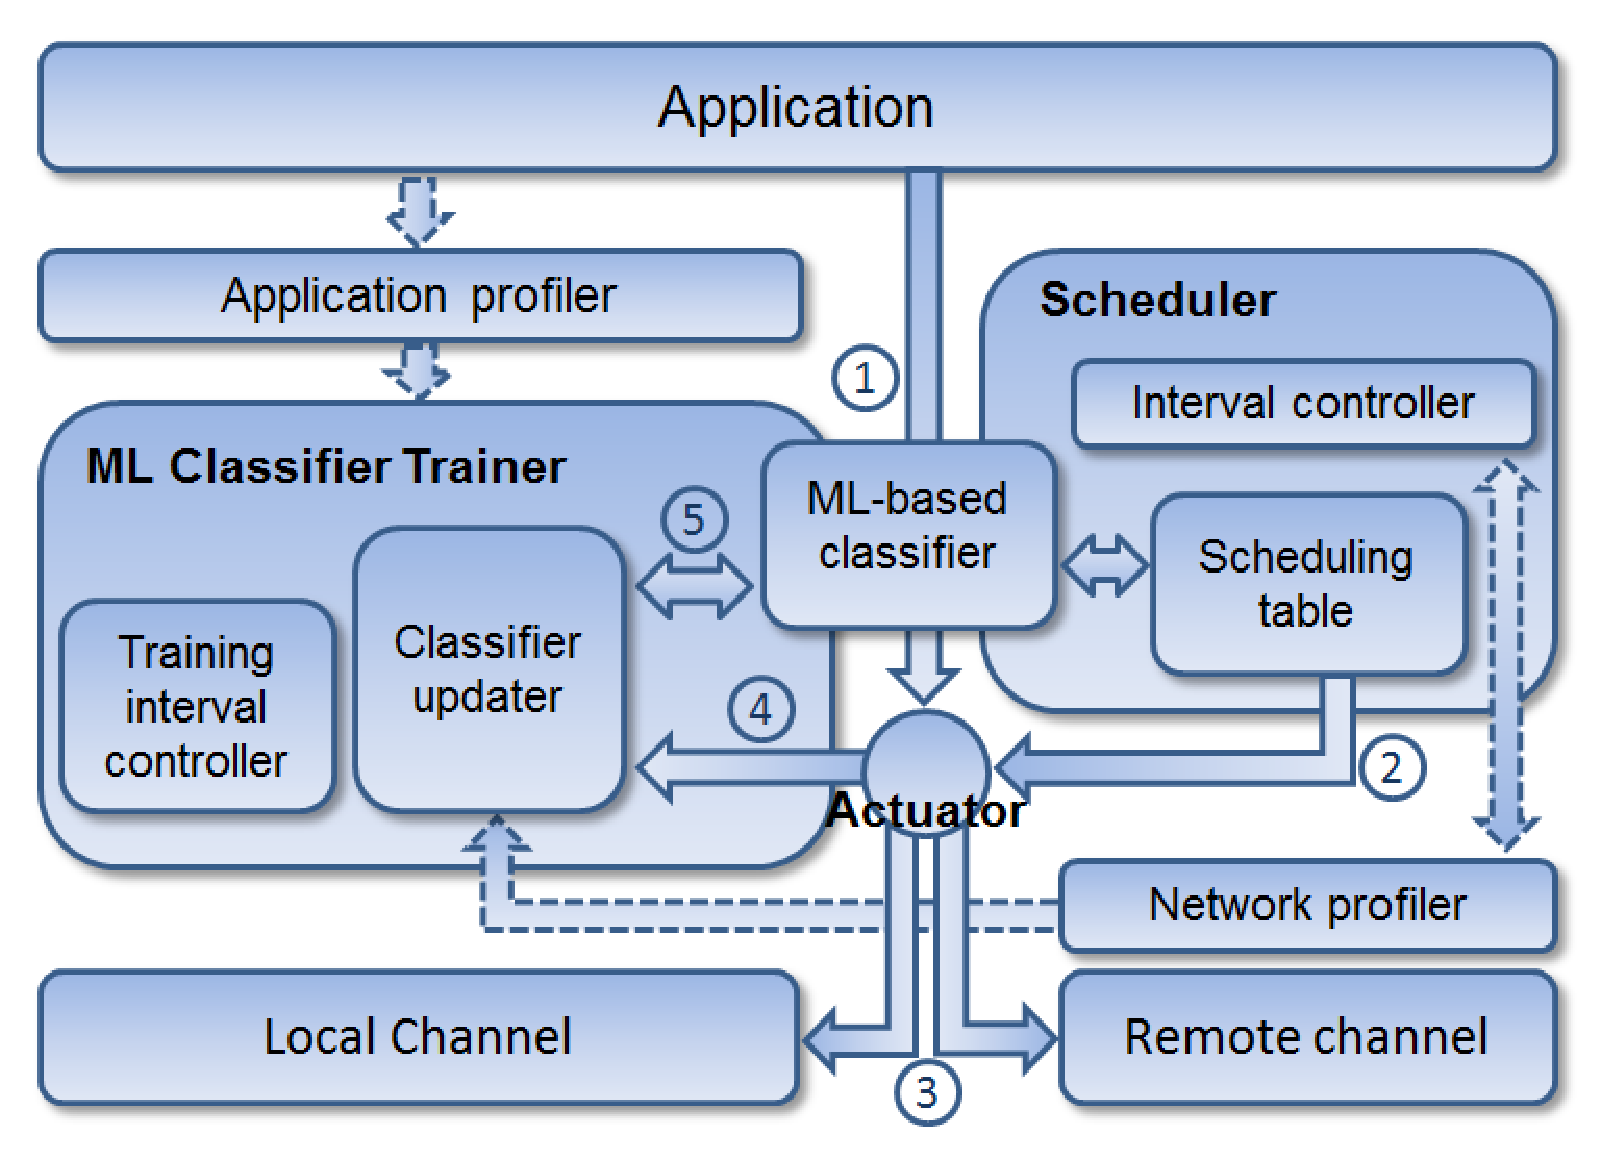
\includegraphics[height=5.1cm, width=7.6cm]{Figure/figure1}
\caption{Overall architecture of MALMOS with online training. The dotted
lines indicate the application and network features flow path, and the
solid lines are the application computing tasks or scheduling-related
commands flow path.}
\end{figure}
%
\subsection{Architecture and Modules of MALMOS}
%\subsection{Architecture of the Machine Learning-based Mobile Offloading
%Scheduler}
%
As depicted in Figure 1, the overall architecture consists
of four main modules: computation dispatcher, runtime scheduler, machine
learning classifier, and the trainer for the machine learning classifier.
%
These four main modules interact with each other to execute and
schedule offloadable tasks, and to train the machine learning
classifier. 
%
At runtime, the system operates in either of two different phases:
\textit{normal operation phase} and \textit{online training phase}.
%
In the normal operation phase, first, the computation dispatcher
receives an offloadable computation (\textcircled{1}).
%
Then, according to the decision provided by the scheduling module
(\textcircled{2}), it forwards this computation to the appropriate
execution unit (\textcircled{3}): either a local computing unit, or a
remote computing unit (through the network interface).
%
In contrast, in the online training phase, the offloadable
computation is forwarded to \textit{both} execution units; the
computation dispatcher records the performance of both, and feeds back
the comparison between offloading and local processing to the trainer
(\textcircled{4}).
%
Based on the feedback from the dispatcher, the classifier trainer updates
the machine learning classifier ({\textcircled{5}).
%
The implementation details for these modules are as follows:\\
%
\textbf{Computation dispatcher.} This module has the
responsibility to forward offloadable tasks either to the
network interface (for offloading) or to the local computing units (for
local processing) according to the scheduling status of each offloadable
computation stored in scheduling table.
%
In the online training phase, this module provides feedback to the
classifier updater in the machine learning classifier trainer module, by
comparing the performance between offloading and local processing and
recording the approach that leads to best performance.\\
%
\textbf{Runtime scheduler.} Scheduling offloadable computations
requires the profiling of internal and external dynamic features, such
as data size of inputs to the task and network latency and bandwidth
conditions which itself results in additional costs in terms of runtime
overhead and energy consumption.
%
Thus, there exists a trade-off between the scheduling performance and
cost: as coarse-grained scheduling is cheaper than frequent
scheduling, but can lead to worse scheduling accuracy.    
%
For this reason, we consider two scheduling strategies.
%
In the first strategy, each time offloadable tasks are called from the
mobile application, the runtime scheduler makes offloading decisions for
each task.
%
We refer to this strategy as \textit{on-demand scheduling}.
%
Another strategy is the \textit{periodic scheduling}, in which the
scheduler makes offloading decisions asynchronously with actual
executions of offloadable tasks, but periodically with a certain
interval.
%
Also, in the periodic scheduling strategy, the scheduling interval
increases and decreases dynamically according to network conditions in
order to prevent unnecessarily frequent scheduling processes.
%
If the variation of network bandwidth is less than a threshold, which
can be thought as the stable network status, the scheduling interval 
becomes longer (i.e. as twice as current interval), because we assume it
is likely that former scheduling can be still effective for the near
future under the stable network condition.
%
In contrast, if the variation of network bandwidth is greater than the
threshold, the interval becomes the half of the current interval leading
more frequent scheduling.
%
To end this, the scheduling interval controller stores a time series
with a history of the previous \textit{N} network bandwidth
measurements.
%
Based on the observation, we set the minimum (also, initial)
and maximum interval to 5 and 20 seconds, respectively.
%
Also, we setup the network variation threshold to 10\% of mean value of
the previous 10 network bandwidth measurements.\\
%
\textbf{Machine learning classifier.} The machine learning classifier is
in charge of making decisions on offloading or local processing for
offloadable tasks by using the attributes obtained by
the network and application profiler, and it stores the scheduling
result to the scheduling table in the scheduler module.
%
Even though it is possible to adopt various attributes
from internal (application) and external (network, remote resources)
environments, for the current implementation, we employ two attributes:
the size of data to be sent to the remote resource, and the network
bandwidth.
%
Note that, in the periodic scheduling strategy in which the scheduler
makes decisions periodically regardless of the calls of offloadable
mobile computations, the application profiler has to estimate the data
size of offloading computations to make offloading decisions, because
the actual data size is not available before the computations are
called.
%
For doing this, the application profiler predicts the possible range of
the data size for each computation using the mean($\mu_{data}$)
and standard deviation($\sigma_{data}$) of previous 10 data size
measurements ($\mu_{data}$-$\sigma_{data}$ $\sim$ $\mu_{data}$+$\sigma_{data}$).
%
Then, the machine learning classifier makes two decisions with maximum
and minimum boundary of the predicted range of data size, and offloading
is scheduled only when two decisions agree on offloading.\\ 
%
\textbf{Machine learning classifier trainer.} With the feedback on the
performance comparison between offloading and local processing from the
computation dispatcher, the machine learning classifier trainer updates
the machine learning classifier.
%
In order to compare the performance between offloading and local
processing, the trainer creates one separate thread for local
processing, so that offloading and local processing can be executed
concurrently.
%
Then, the computation dispatcher measures the execution time for both
offloading and local processing to compare the performance and provides
the comparison result to the classifier updater. 
%
Finally, the classifier updater trains the machine learning classifier 
with the feedback from the computation dispatcher and the attributes
from the profilers.
%
%
\begin{figure}
\algsetup{indent=1.0cm}
\begin{algorithmic}[1]
\STATE{\textit{$//$ switch the training and normal operation phase}}
\WHILE{$one$ $period$ $is$ $NOT$ $finished$}
	\IF{$it$ $is$ $in$ $normal$ $operation$ $phase$}
		\STATE {$do$ $scheduling$}
	\ELSE
		\IF{$accu_{curr}$ $is$ $higher$ $than$ $th_{accu}$}
			\STATE{$switch$ $normal$ $operation$ $phase$}
		\ELSE
			\STATE{$stay$ $training$ $phase$}
		\ENDIF
	\ENDIF
\ENDWHILE
\STATE
\STATE{\textit{$//$ calculate the length of the next period}}
\IF{$errors$ $happened$}
	\STATE{$period_{next}$$\gets$$period_{curr}$$-$$($$period_{min}$$\times$$n_{err}$ $)$}
\ELSE
	\STATE{$period_{next}$$\gets$$period_{curr}$$+$$period_{min}$}
\ENDIF
\end{algorithmic}
\caption{Adaptive online training mechanism}
\end{figure}
%
\subsection{Adaptive Online Training Mechanism}
%
One of the main contributions of this work is the adaptive online
training mechanism which allows the training phase duration to stretch
and shrink dynamically according to the scheduling accuracy.
%
The pseudo-code of the adaptive online training mechanism is shown in
Figure 2.
%
First, line 2$\sim$12 decide to switch the training and normal operation
phase by calculating the current scheduling accuracy.
%
In the training phase, if the current accuracy ($accu_{curr}$) is higher
than the accuracy threshold ($th_{accu}$), the online training mechanism
switches to the normal operation phase.
%
Otherwise, it stays in the training phase.
%
Next, the length of the next period is calculated according to the
number of incorrect decisions (line 15$\sim$19).\\
%
\indent Figure 3 illustrates an example of how the adaptive online
training mechanism works.
%
In this example, we set the accuracy threshold ($th_{accu}$) to 70\% and
the minimum length of one period to 5.
%
Also, we assume that there is no incorrect decision or scheduling error
in the first, second, and fourth period, but one error in the third
period.
%
In order to measure the current scheduling accuracy ($accu_{curr}$) of
the classifier, the trainer observes whether the performance comparison
matches with the offloading decision.
%
For example, if the classifier makes a decision to offload and
offloading actually has better performance than local processing, we
regard this case as a correct decision.
%
Then, we calculate the current scheduling accuracy using Equation 1.
%
\begin{equation}
	accu_{curr} = N_{correct}\:/\:(N_{total} + 1)
\end{equation}
%
where $N_{correct}$ and $N_{total}$ are the number of correct decisions
and total decisions.
%
Also, we added one to the denominator in order to avoid 100\% of
scheduling accuracy at just one training (if the decision is correct in
the first training turn, the scheduling accuracy becomes 100\%).\\
%
\indent In Figure 2, the normal operation phase begins after three
training turns in the first and second period because the scheduling
accuracy at third training turn is 75\% which is higher than 
$th_{accu}$, 70\%.
%
% Heungsik: why do you increase by a constant? why decrease by period times #errors?
% you are describing the mechanism without providing much justification for your
% choices, or guidance as to how to pick up values for thresholds, etc. 
Furthermore, because there was no decision error in the first and second
period, the next length of one period carefully increases by adding the
minimum length of one period, thus, the length of the second and third
period becomes 10 and 15, respectively.
%
In the third period, however, as one incorrect decision has been
occurred, the training phase holds for six executions when the
scheduling accuracy becomes higher than 70\%, and the length of the
fourth period decreases by the minimum length of one period multiplied
by the number of incorrect decisions (int this case, 1).
%
For this adaptive online training mechanism, we borrowed the concept of
the feedback control algorithm used for TCP congestion avoidance called
\textit{Additive Increase Multiplicative Decrease}.
%
\begin{figure}
\centering
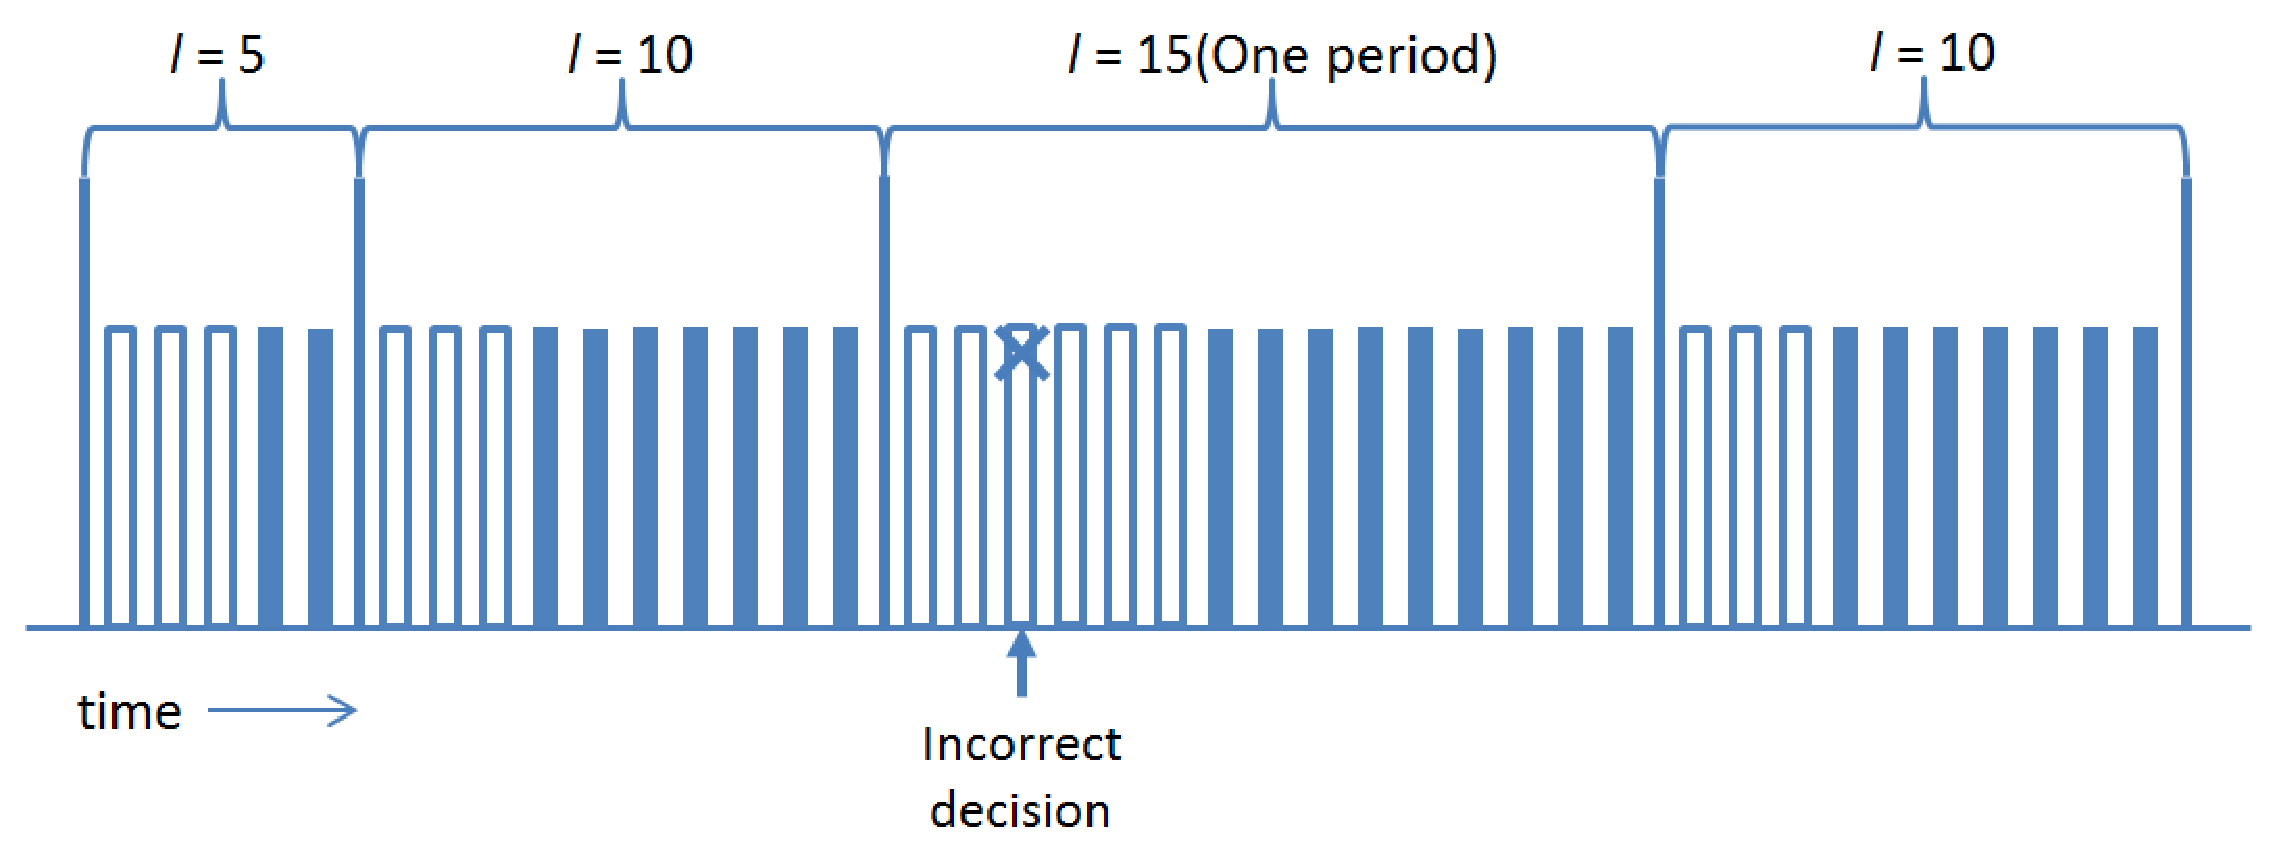
\includegraphics[height=3.3cm, width=8.5cm]{Figure/figure2}
\caption{An example of the adaptive online training mechanism. For this
example, we set 70\% of the scheduling accuracy threshold and 5 of the
minimum number of the mobile computation executions.}
\end{figure}
%
\subsection{Integration with On-Demand Java-based Offloading Framework}
%
To demonstrate the applicability of this approach, we integrated the
modules of MALMOS into the DPartner mobile application framework, which
is capable of automatically refactoring Java-based mobile applications
to identify offloadable computation tasks.
%
Given an Android mobile application, first of all, DPartner examines its
bytecode to classify the Java classes into the anchored and offloadable
classes, so it can be guaranteed that the anchored classes are executed
on the mobile device while directly using a variety of the local sensors
such as the GUI display, camera, accelerator, and GPS.
%
Also, DPartner rewrites the bytecode for the offloadable classes to
implement a special type of the program structure to support on-demand
offloading.
%
Then, DPartner packages the files such as images, xml files, external
libraries, and rewritten bytecode for the offloadable classes, and
generates two separate objects which are deployed into the mobile device
and the remote server, respectively.\\
%
\indent With respect to scheduling, however, the offloading-capable
Android applications generated by DPartner requires either static or
user-provided decisions. 
%
However, static scheduling becomes inaccurate if conditions change, and
it is impractical that the mobile user monitors the internal and
external environments and schedules each offloadable mobile computations
at runtime.
%
We address this challenge by integrating MALMOS with the
offloading-capable mobile applications generated by DPartner. 
%
We were able to achieve this integration without requiring deep
modifications or code additions to DPartner.
%
In fact, the only major code addition is to define new APIs to acquire
the data size of offloadable computations and the network bandwidth. 
%
By combining MALMOS with these applications, the mobile user can be free
of the burden of the scheduling tasks.
%
\section{Evaluation}
%
In this section, we evaluate the implementation of MALMOS with
respect to the scheduling accuracy and classifier training cost.
%
In order to compare the performance and cost among the different
categories of machine learning algorithms, we utilize three machine
learning algorithms: instance-based learning, single layer perceptron,
and na\"{i}ve bayes.
%
\begin{figure*}[ht]
\centering
\subfigure[Training time] {
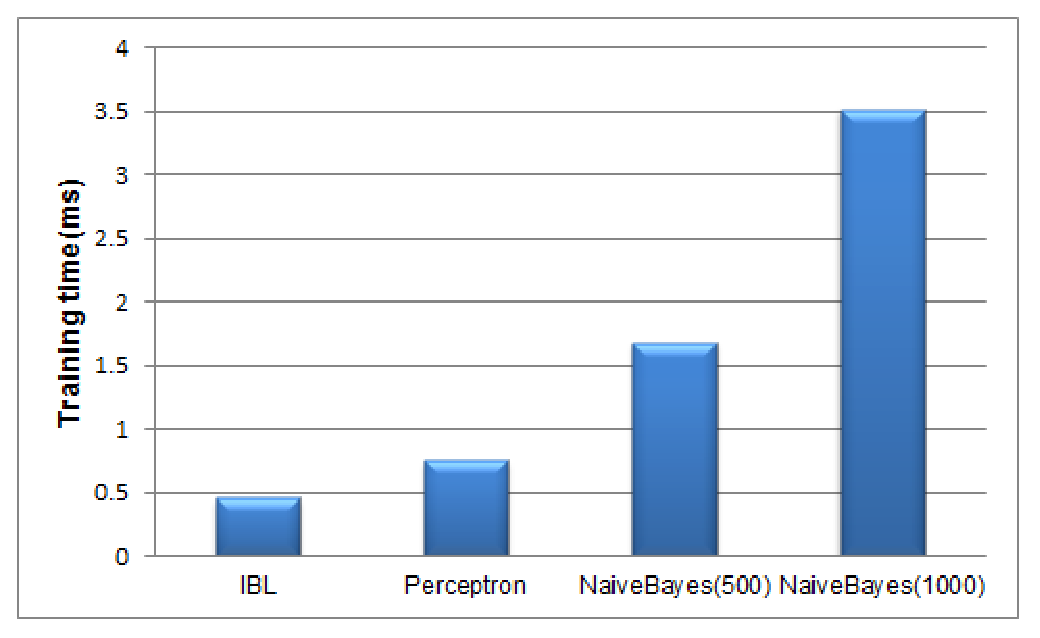
\includegraphics[height=4.0cm, width=5.6cm]{Figure/figure4}
}
\subfigure[Classification time] {
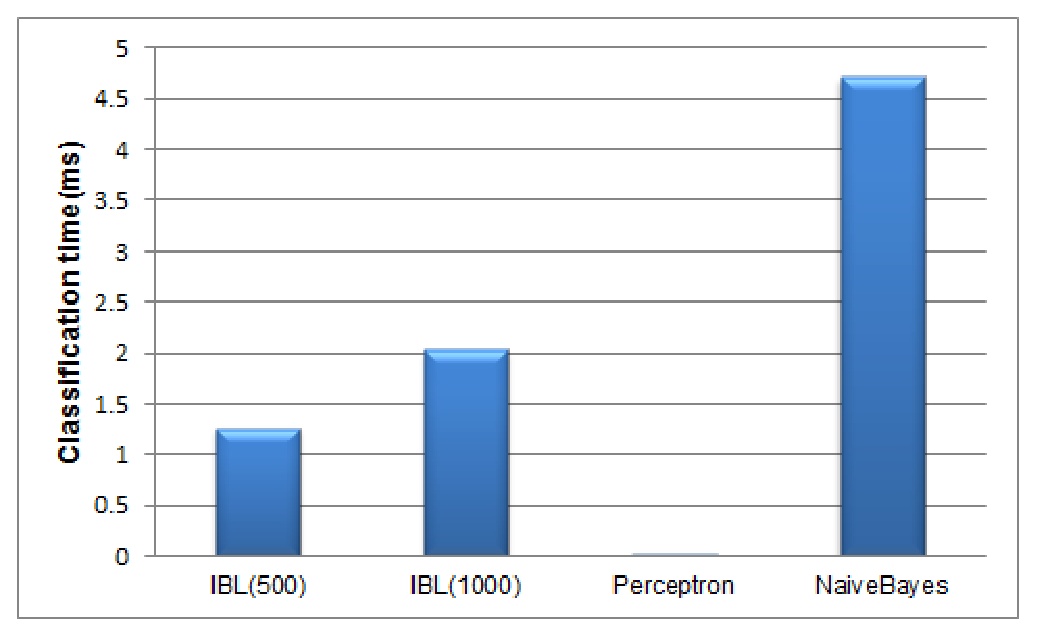
\includegraphics[height=4.0cm, width=5.6cm]{Figure/figure5}
}
\subfigure[Scheduling accuracy] {
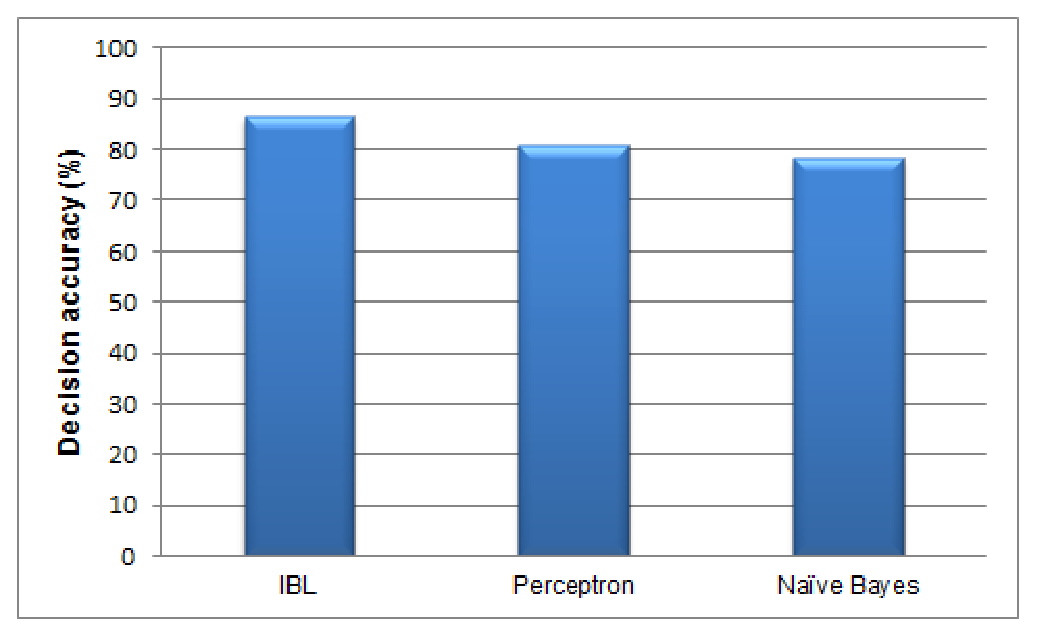
\includegraphics[height=4.0cm, width=5.6cm]{Figure/figure6}
}
\caption{Performance and cost comparison for three machine learning
algorithms}
\end{figure*}
%
\subsection{Experimental Setup}
%
Even though high dimensional machine learning algorithms such as
decision tree, multilayer perceptron, and support vector machine can
achieve more accurate scheduling performance, they might be too
expensive to be used for the mobile offloading scheduler.
%
Based on the intuitive observation on the algorithm complexity, we
selected three machine learning algorithms: instance-based learning,
single layer perceptron, and na\"{i}ve bayes.\\ 
%
\indent Our hardware setup consists of the mobile client and
remote server which are connected through a wireless router.
%
We have utilized an Android tabletPC, Nexus 5 equipped with 2.3GHz
quad-core processor and 2GB RAM, and running Android KitKat as the
mobile client.
%
For the remote server, we used a workstation with Intel 3.0GHz Core2 Duo
processor and 8GB memory which is running Linux OS.
%
In order to emulate various network conditions, furthermore, we
configured different network bandwidth using Traffic Control
(TC)~\cite{tc}, a network tool which provides functionality to control
network traffic by prioritizing network resources and using concepts of
traffic classification, queue disciplines, and quality of service.
%
Also, for the mobile application used in the evaluation, we created
a synthetic benchmark application, matrix multiplication, and DPartner
rewrote it as the offloading-capable application.
%
Though, theoretically, DPartner is applicable to any types of Android
mobile applications, it is not possible to intentionally change the data
size and the amount of computation for the real-world applications.
%
With matrix multiplication, we are able to easily vary the data size and
the amount of computation by manually controlling the matrix size.
%
\subsection{Overhead of training and classification}
%
Since our machine learning-based mobile offloading scheduler keeps
training the classifier, which leads some runtime overhead, we
observed the cost to train the machine learning classifier.
%
As shown in Figure 4(a), instance-based learning has the shortest
classifier training time among three machine learning algorithms.  
%
In fact, the basis for the classification of instance-based learning is
the instance database, where previously experienced cases are stored.
%
Instead of training the explicit classifier, therefore, instance-based
learning adds a new instance to the database for the future
classification raising relatively small training overhead.
%
On the other hand, na\"{i}ve bayes with 1000 instances of database has
the worst training overhead. 
%
For the algorithm perspective, na\"{i}ve bayes measures the
probability density for the given classes with the mean and standard
deviation, and chooses the class with the highest probability.
the highest probability.
%
Thus na\"{i}ve bayes calculates the mean and standard deviation
throughout the previous instances for each class whenever a new instance
is trained.
%
Consequently, na\"{i}ve bayes with 1000 instances, which requires
relatively heavy calculations for the mean and standard deviation, has
bigger training overhead than other machine learning algorithms.\\
%
\indent Also, Figure 4(b) shows the classification time that the machine
learning classifier consumes to make a decision.
%
Similarly as the training time, na\"{i}ve bayes shows bigger overhead
than other machine learning algorithms.
%
In fact, we used the Gaussian distribution to calculate the probability
density for each class with the mean and standard deviation value.
%
Therefore, the classification for na\"{i}ve bayes entails the complex
arithmetic operations such as the exponential function and the square root
which take longer than addition, multiplication, or comparison.
%
For that reason, na\"{i}ve bayes has the worst classification overhead.
%
Note that perceptron has remarkably low classification overhead compared
with other machine learning algorithms. 
%
For perceptron, the classification process involves calculating the
output from a multivariable linear equation consisting of the attributes
weighted by the coefficients, which requires the insignificant amount of
the computation. 
%
As a result, perceptron shows the lowest cost in terms of the
classification time amongst three machine learning algorithms.
%
\subsection{Scheduling Accuracy}
%
We also investigated the scheduling accuracy of three machine learning
algorithms.
%
For the unbiased evaluation, we turned off the adaptive online training
mechanism and the training phase and normal operation phase were
uniformly switched in one period (5 trainings and 15 normal operations)
and 10 periods were repeated for the average.
%
Also, in order to observe the impact of the dynamic network condition
and data size on the scheduling accuracy, we changed the network
bandwidth randomly among 1MB/s, 2.5MB/s, 5MB/s, and 9.5MB/s with
a same interval and each computation processes the different matrix size
having the different data size. 
%
In this experimental setup, we observed how accurate each machine
learning makes decisions in the normal operation phase.\\
%
\indent As you can see in Figure 4(c), instance-based learning achieves
the highest scheduling performance, showing 87\% of the scheduling
accuracy.  
%
As we mentioned earlier, instance-based learning compares a new
scheduling problem with the all of the stored instances in the database
to find out the most similar case in the database.
%
It is because that instance-based learning can hardly miss any
information from the previously stored instances.
%
On the other hand, na\"{i}ve bayes has the worst scheduling accuracy
which is lower than 80\% of the accuracy.
%
The reason is that the classification of the probabilistic machine
learning algorithms is based on the statistics of attributes of the
previous instances such as the mean and standard deviation.
%
Thus it is possible that the probability-based machine learning
algorithms can overlook the edge of previously seen instances, which
causes the performance degradation for the prediction problem.
%
\section{Use Case}
%
We applied our machine learning-based mobile offloading scheduler with
online training to Go, the two players board game which is available in
Google Play.
%
In Go game shown in Figure 5, the next stone position of the competitor
is calculated through the Monte Carlo tree search algorithm, thus the
offloading-capable version of the Go game offloads the Monte Carlo
algorithm to the remote server according to the board size and network
bandwidth.
%
Also, for Go game, the quick reactivity from the competitor is one of
the important aspects to play the game seamlessly.
%
So, the on-demand scheduling strategy can cause relatively high overhead
by doing the scheduling process for every competitor turn.
%
For that reason, we utilized the periodic scheduling strategy for Go
game.\\
%
\indent Another possible application is the optical character
recognition (OCR) application with the translation between different
languages.
%
Character recognition and language translation technologies include
the complex mechanisms such as pattern recognition and data mining which
are suitable for offloading.
%
Hence, the flexibility of where to execute these complex algorithms
according to the image size and network conditions will help the mobile
device improve the performance and save energy consumption.
%
%\begin{figure}
%\centering
%
\includegraphics[height=5.0cm, width=4.0cm]{Figure/figure7}
%\caption{Go game generated by DPartner.}
%\end{figure}
%
\section{Conclusion and Future Work}
%
In this paper, we proposed the machine learning-based mobile offloading
scheduler with online training, MALMOS.
%
First, we modularized MALMOS to generally apply to any types of mobile
offloading frameworks.
%
Also, we suggested the adaptive online training mechanism in which the
training phase and normal operation phase are dynamically switched
according to the scheduling accuracy.
%
To evaluate our work, we applied MALMOS to the Java-based on-demand
offloading framework.
%
Also, we utilized three different machine learning algorithms for the
offloading scheduler and compared the overhead and performance in terms
of the training time, classification time, and scheduling accuracy.
%
In the evaluation, we observed that instance-based leaning and
perceptron have higher than 80\% of the scheduling accuracy with the
reasonable overhead.\\
%
\indent For the future work, we plan to apply our work to various types
of mobile offloading frameworks with more machine learning algorithms
and target real-world applications.
%
\begin{figure}
\centering

\includegraphics[height=5.0cm, width=4.0cm]{Figure/figure7}
\caption{Go game generated by DPartner.}
\end{figure}
%
\section*{Acknowledgment}
This material is based upon work supported in part by the National Science
Foundation under Grant No. 0910812, 0758596, 0855031, 1265341, and
1339737.
%
Any opinions, findings, and conclusions or recommendations expressed in
this material are those of the author(s) and do not necessarily reflect
the views of the National Science Foundation.
%
%\bibliographystyle{IEEEtran}
\bibliography{ipccc14}
\end{document}


